\documentclass[11pt, a4paper]{article}

\usepackage{style}

\author{Vladislav Mlejnecký}

\title{%
  Číslicové zpracování signálů\\
  \large Úloha číslo 1.\\
  Generování a vykreslování signálů v prostředí Matlab}

\begin{document}

    \maketitle
    
    \pagenumbering{arabic}

    \section{Zadání}
        \begin{enumerate}
            \item
            generujte, nakreslete vhodnou část průběhu a přehrejte 0,5 sekundy dlouhý harmonický signál o frekvenci 400 Hz a vzorkovací frekvenci 8kHz
            \item
            generujte a zobrazte  4 periody harmonického signálu o frekvenci 400 Hz a vzorkovací frekvenci 8kHz
            \item
            generujme a zobrazte 25 vzorků harmonického signálu o frekvenci 400 Hz a vzorkovací frekvenci 8kHz
            \item
            generujme a zobrazte jednotkový impulz  (digitální obdoba Diracova impulzu), 
            \item
            generujme a zobrazte jednotkový skok
            \item
            vytvořte a zobrazte signál složený postupně ze dvou period signálu o frekvenci 50Hz, čtyř period o frekvenci 100Hz a opět dvou period 50Hz, vzorkovací frekvence 8kHz
            \item
            vytvořte a zobrazte 4 periody signálu pilovitého průběhu o frekvenci 400 Hz, vzorkovací frekvence 8kHz
        \end{enumerate}
    
    \section{Výsledné grafy}
    
        \begin{figure}[H]
            \centering
            \begin{minipage}{.5\textwidth}
                \centering
                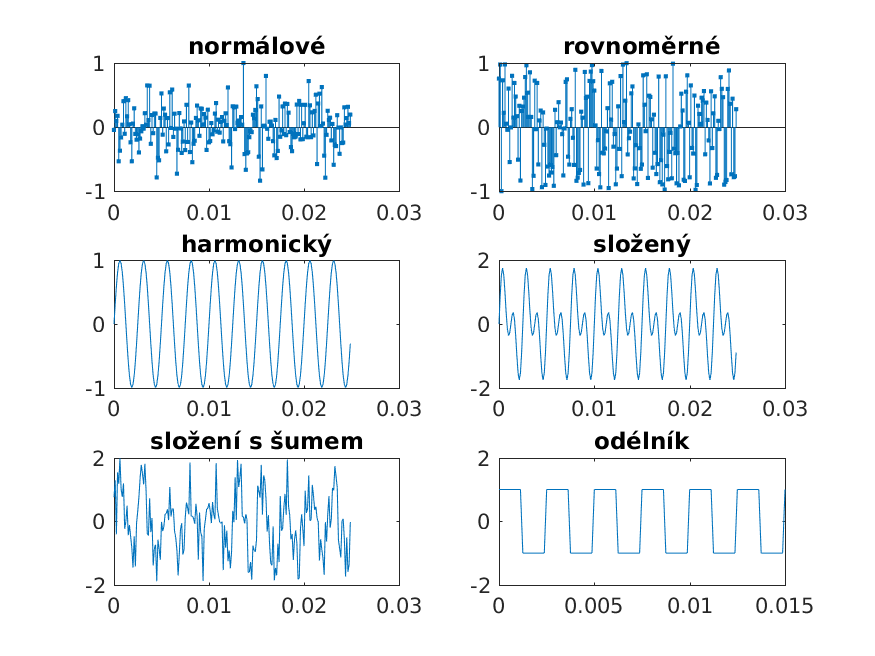
\includegraphics[width=.9\textwidth]{matlab/1.png}
                \caption{Harmonický signál}
                \label{fig:graf1}
            \end{minipage}%
            \begin{minipage}{.5\textwidth}
                \centering
                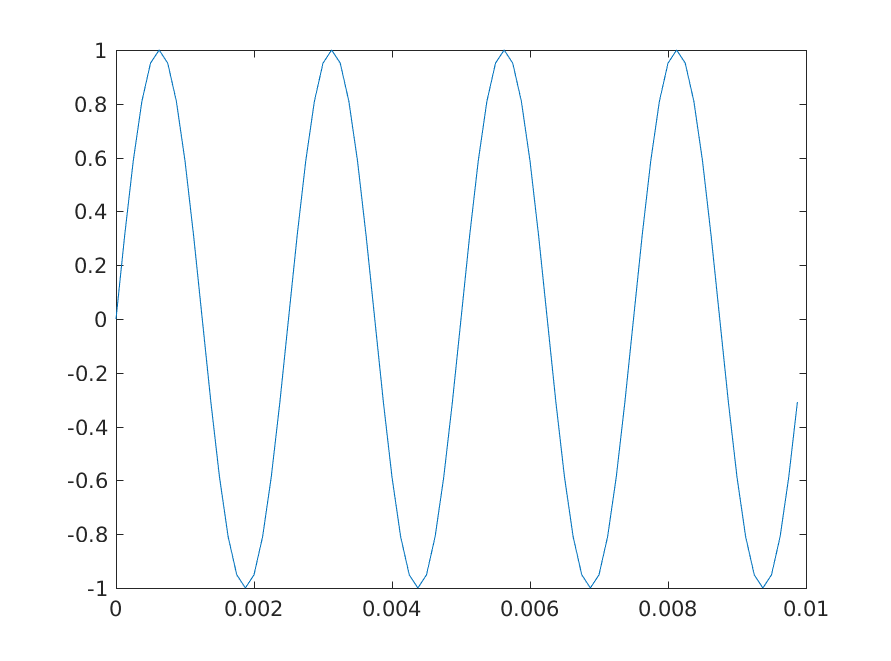
\includegraphics[width=.9\textwidth]{matlab/2.png}
                \caption{25 vzorků signálu}
            \label{fig:graf3}
            \end{minipage}
        \end{figure}

        \begin{figure}[H]
            \centering
            \begin{minipage}{.5\textwidth}
                \centering
                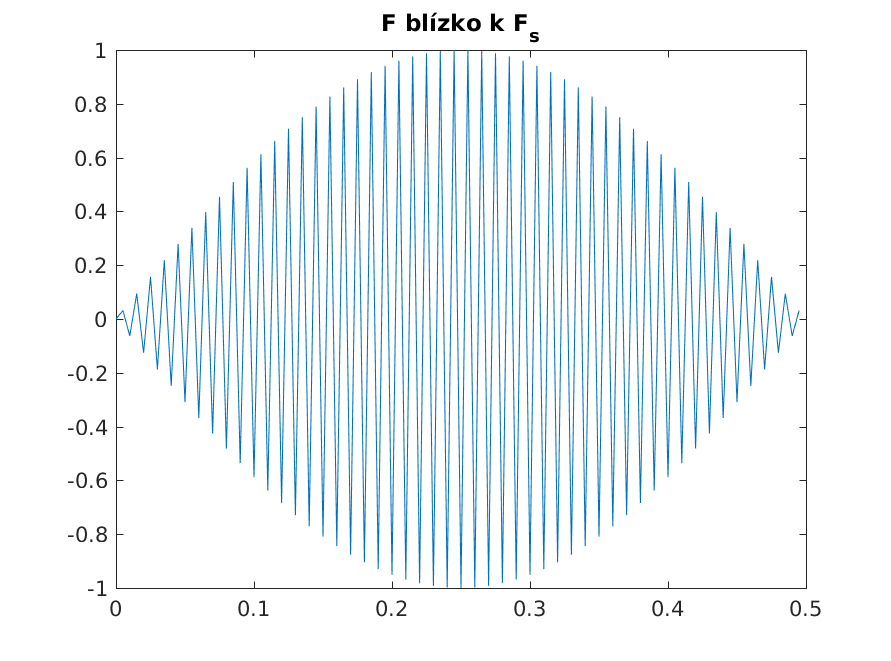
\includegraphics[width=.9\textwidth]{matlab/3.png}
                \caption{25 vzorků signálu}
                \label{fig:graf3}
            \end{minipage}%
            \begin{minipage}{.5\textwidth}
                \centering
                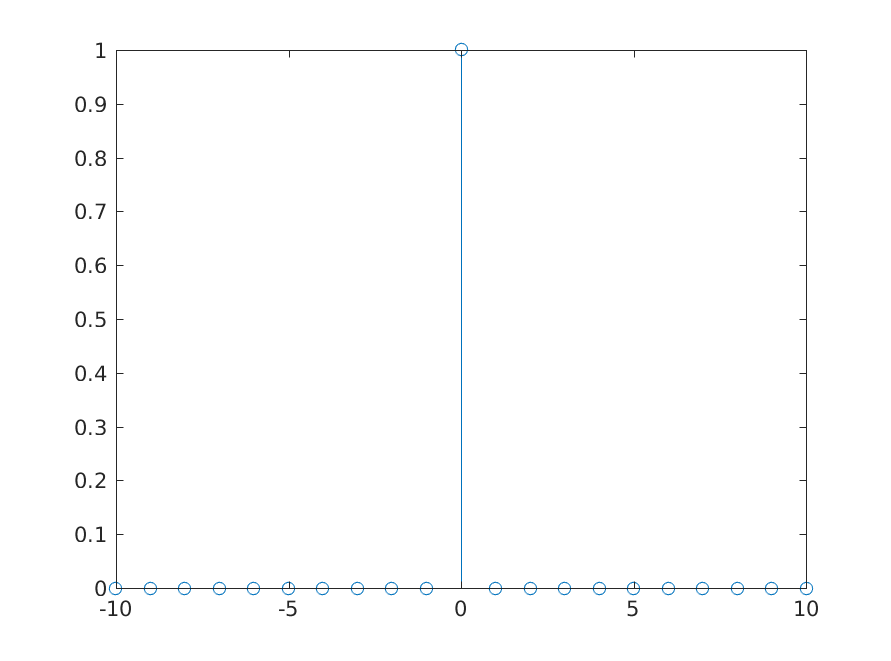
\includegraphics[width=.9\textwidth]{matlab/4.png}
                \caption{Jednotkový impulz}
                \label{fig:graf4}
            \end{minipage}
        \end{figure}
        
        \begin{figure}[H]
            \centering
            \begin{minipage}{.5\textwidth}
                \centering
                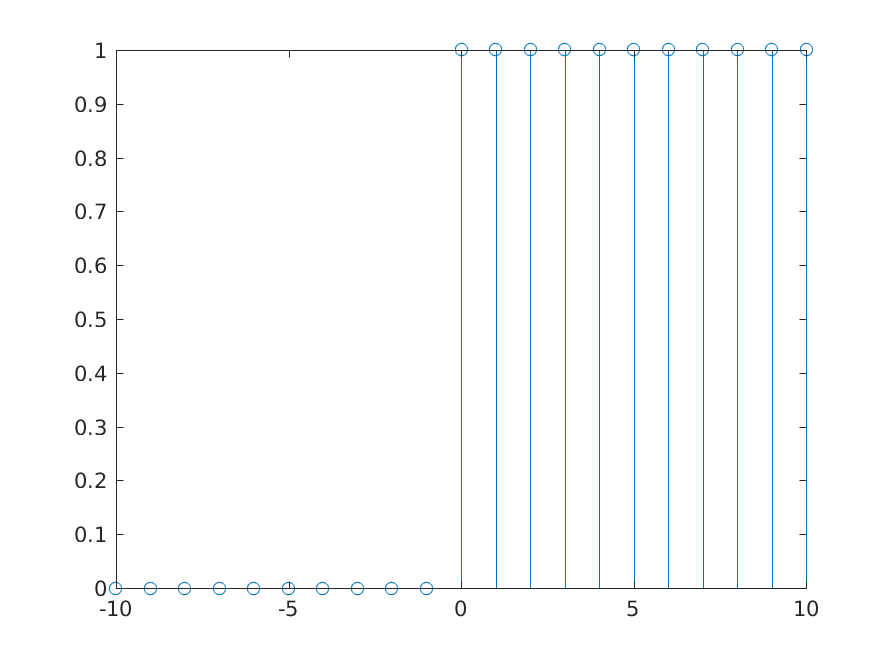
\includegraphics[width=.9\textwidth]{matlab/5.png}
                \caption{Jednotkový skok}
                \label{fig:graf5}
            \end{minipage}%
            \begin{minipage}{.5\textwidth}
                \centering
                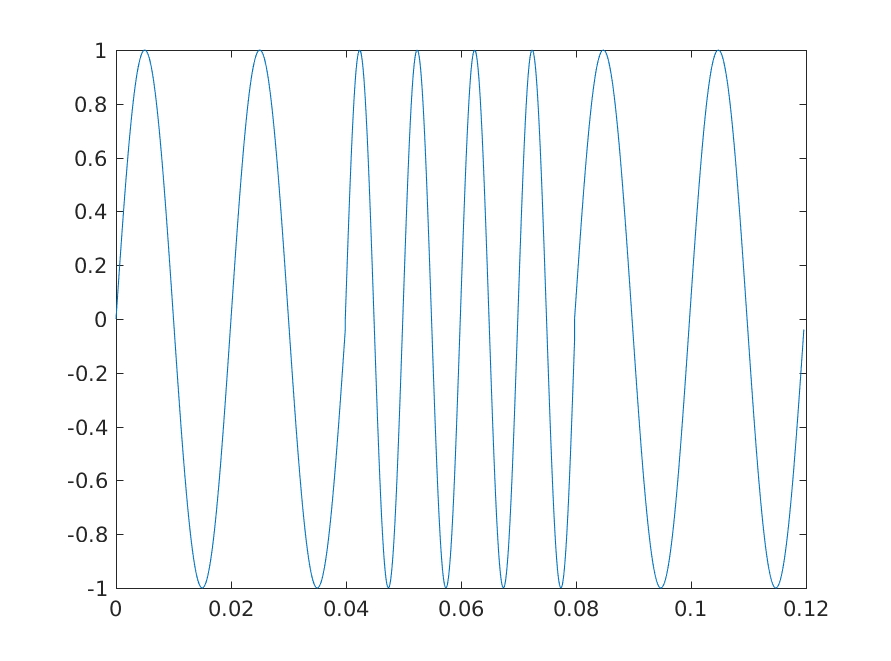
\includegraphics[width=.9\textwidth]{matlab/6.png}
                \caption{Složený signál}
                \label{fig:graf6}
            \end{minipage}
        \end{figure}
        
        \begin{figure}[H]
            \centering
            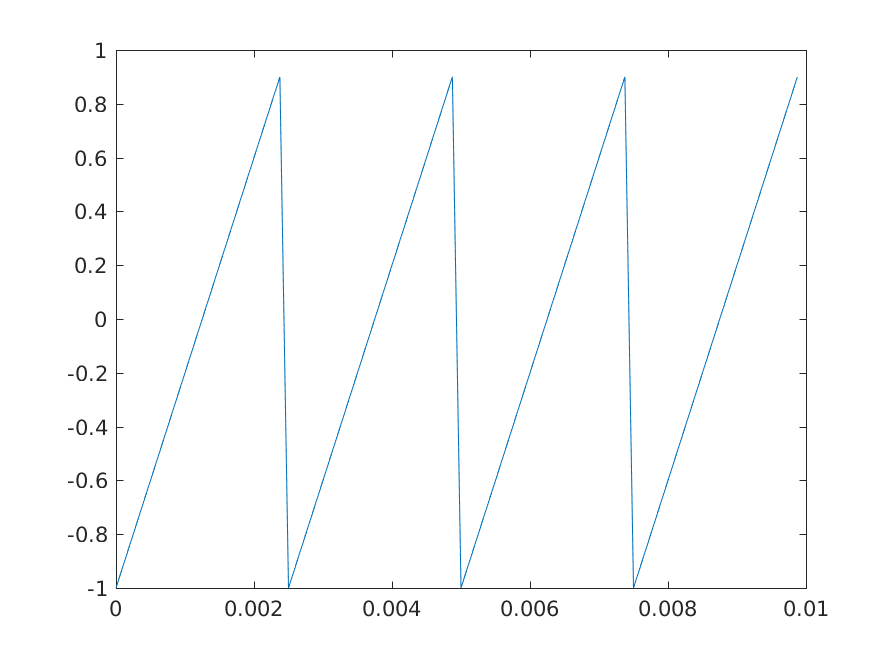
\includegraphics[width=.5\textwidth]{matlab/7.png}
            \caption{Pilový průběh}
            \label{fig:graf7}
        \end{figure}
    
    \section{Výpis zdrojového kódu}
    
\begin{lstlisting}[language=matlab, frame=single]
Fs = 8000;                                         

t = 0:1/Fs:0.5-1/Fs;                              
y1 = sin(2 * pi * 400 * t);                       
h1 = plot(t(1:length(t)/25), y1(1:length(y1)/25));
sound(y1, Fs);                                    
saveas(h1, '1.png');                              

t = 0:1/Fs:4/400 - 1/Fs;
y2 = sin(2 * pi * 400 * t);
h2 = plot(t, y2);
saveas(h2, '2.png');

t = (0:24)/Fs;
y3 = sin(2 * pi * 400 * t);
h3 = stem(t, y3); 
saveas(h3, '3.png');

n = -10:10;
y4 = n == 0;
h4 = stem(n, y4);
saveas(h4, '4.png');

n = -10:10;
y5 = n >= 0;
h5 = stem(n, y5);
saveas(h5, '5.png');

t1 = 0:1/Fs:2/50 - 1/Fs;
t2 = 0:1/Fs:4/100 - 1/Fs;
y6 = sin(2 * pi * 50 * t1);
y6 = [y6 sin(2 * pi * 100 * t2)];
y6 = [y6 sin(2 * pi * 50 * t1)];
t = t1; 
t = [t (t2 + t1(length(t1)))];
t = [t (t1  + t2(length(t2)) + t1(length(t1)))];
h6 = plot(t, y6);
saveas(h6, '6.png');

t = 0:1/Fs:4/400 - 1/Fs;
y7 = sawtooth(2 * pi * 400 * t);
h7 = plot(t, y7);
saveas(h7, '7.png');
\end{lstlisting}


\end{document}
